\begin{table*}[t]
	\caption{FET performance on CHEMET}
	\centering
	\label{table:result}
% 	\begin{small}
			\begin{tabular}{cllllll}
				\toprule
				\multirow{2}{*}{\textbf{Model}} 
				& \multicolumn{3}{c}{\textbf{Dev}} 
				& \multicolumn{3}{c}{\textbf{Test}} \\             
				& \textbf{Accuracy} & \textbf{Macro F1} & \textbf{Micro F1} & \textbf{Accuracy}&  \textbf{Macro F1} & \textbf{Micro F1} \\  
				\midrule
				BioBERT & 1 & 2 & 3 & 1 & 2 & 3 \\      
				SciBERT & 1 & 2 & 3 & 1 & 2 & 3 \\ 
				FETBSL1& 1 & 2 & 3 & 1 & 2 & 3 \\ 
				FETBSL2 & 1 & 2 & 3 & 1 & 2 & 3 \\ 
				Our Model & 1 & 2 & 3 & 1 & 2 & 3 \\ 
				\bottomrule    
			\end{tabular}
		
% 	\end{small}
\end{table*}
% 	\end{small}
\begin{table}[t]
	\begin{small}
	\caption{Ablation Study}
	\centering
	\label{table:ablation}
			\begin{tabular}{lll}
				\toprule
				\textbf{Model}
				& \textbf{Macro-F1} & \textbf{Micro-F1}  \\  
				\midrule
				
				Full Model& 1 &2 \\\hline 
				w/o description& 1 &  \\      
				w/o graph& 1 &2  \\    
				w/o cross-modal attention& 1 &2  \\       
				w/o context-only repr.& 1 &2  \\   
				\bottomrule    
			\end{tabular}
		
	\end{small}
\end{table}

% \begin{table}
% 	\caption{Dataset Statistics for CHEMET}
% 	\centering
% 	\begin{tabular}{lllll}
		
% 		\toprule
% 		Setting &Anno.& \#Inst. & \#Mention  & \#Types \\
% 		\midrule
% 		Train &Distant&   8000& NA&43\\
% 		Dev &Human&1000&NA&NA\\
% 		Test&Human&            1000&NA&NA \\
% 		\bottomrule
% 	\end{tabular}
% 	\label{datastats}
% \end{table}
%  to our knowledge
\section{Experiments}
\label{sec:experiment}
Since there is no other fine-grained chemical entity typing datasets, we evaluate fine-grained chemical entity typing on CHEMET. The experiments can be reproduced using implementations provided in Appendix~\ref{appendix2}.
\subsection{Baseline Methods}
% \cheng{It would help to clarify what questions we can answer by comparing the proposed methods with these baselines. It seems to me that these baseline methods do NOT use the same amount of information/resources as the proposed method. If so, the improvement may have come from the fact that we have used additional information/resources, which wasn't used in the baseline methods. This wouldn't be a surprising finding as we are expected to do better with more resources/information. The more interesting question here is: what's the best way of exploiting such information? So if possible, it would be great to include stronger baseline methods that use the SAME amount of extra information. This would help showing the proposed  method is better, not just because it has access to more information/resources, but also because the method can better utilize the extra information than a baseline way of using it (e.g., straightforward combination of existing methods to achieve the goal). Ideally, the baseline methods can be aligned with the most relevant previous work discussed in the related work section. This would help us empirically examine/support the novelty of the work in comparison with previous work from multiple perspectives (e.g., the perspective of tackling the complex name mentions, the perspective of multi-modal attention/embedding, and the connection between local context with molecule structure(?). }
 In the experiment, we compared our method with the following state-of-the-art baselines,
%(NER) 

\noindent \textbf{SciBERT}. SciBert~\cite{scibert} is a Transformer based language model pretrained on sample of 1.14M papers from Semantic Scholar, in which 82\% are from the broad biomedical domain. A linear layer is applied on the embedding of the marker ``*'' embedding for classification.

\noindent \textbf{SciBERT-D} and \textbf{SciBERT-G}. Based on Scibert, we also create variants that additionally use either description sentences (D) or chemical structure graph (G) as features.

% \noindent \textbf{BioBERT}. Similar to SciBert but pretrained on PubMed abstracts (PubMed) and PubMed Central full-text articles (PMC). Similar to SciBRET, a final linear layer is applied for classification.

\noindent \textbf{Latent Type Representation}. \citet{lin2019attentive} used a hybrid classification method beyond binary relevance to exploit type inter-dependency with latent type representation

\noindent \textbf{Fine-Grained Entity Typing in Hyperbolic Space
} Utilized hyperbolic embeddings. @Nik


%\noindent \textbf{Fine-Grained Entity Typing in Hyperbolic Space}. used Hyperbolic embedding



%\noindent \textbf{Baselines}.
%\noindent \textbf{Implementation}


\subsection{Implementation Detail}

Our model is implemented using PyTorch \cite{pytorch} and Huggingface Transformers \cite{huggingface} with SciBERT as text encoder. We left model parameters and reproducibility details in the appendix. 

\subsection{Result}
Table~\ref{table:result} shows the overall result for developement and test set on CHEMET. We can see that our model achieves a higher performance on F1 than every other baseline. We can see a performance of SciBERT, which only uses the local context, is not as good as other baselines, and this shows the importance of incorporating non-local features, which adds information that assists disambiguating mention types. We can also see a clear increase of performance from SciBERT-D and SciBERT-G from our model, which shows the importance of incorporating multimodal definition for chemical entities in chemistry literature.

\subsection{Ablation Study}
To show the improvement made by each of the submodules in our method, we perform an ablation study on CHEMET developement set and show results in Table~\ref{table:ablation}. For model [w/o graph] and [w/o description], we discard $\mathbf{f}_cm$ and correspondingly $\mathbf{f}_g$ or $\mathbf{d}_\textbf{[CLS]}$. For model [w/o cross-modal attention], we left out $\mathbf{f}_cm$, and For model [w/o context-only repr.], we keep every thing other than $\mathbf{\mathbf{m}_\text{MASK}}$

% we truncate model in the following way

% \begin{itemize}[noitemsep,topsep=0pt]
	
% 	\item w/o multimodal alignment: FFNN
% 	\item w/o molecule graph: 
% 	\item w/o description text: 
% \end{itemize}


\subsection{Cross-Modal Attention Analysis}
We show a heatmap visualization of transformer attention scores (between $[\mathbf{n}_1, \mathbf{n}_2,...]$ and $[\mathbf{d}_1, \mathbf{d}_2,...]$) in Figure~\ref{fig:attn} where lighter color corresponds to higher values. We take an example from the chemical . We show that the text concepts and graph substructure indeed have reasonable correlation with each other.


While we apply multimodal entity representation technique to fine-grained chemical entity typing, the idea can be well generalized to other ChemIE tasks such as relation extraction and reaction event extraction, in which chemical entities play a major role. We will release new datasets on other ChemIE task in the near future.

% maybe change to show example like in tuan zixuan's paper show external knowledge helps


\subsection{Qualitative Analysis}
Here we analyzed the remaining errors and categorize the into different cases  (shown in Figure \ref{error_dist}). We discuss the most common ones below,

% While we applied the multimodal entity representation technique to fine-grained chemical entity typing, the idea can be well generalized to other ChemIE tasks such as relation extraction and reaction event extraction, in which chemical entities play a major role. We will release new datasets on other ChemIE task in the near future.

% \begin{figure*}[ht]
% 	\begin{center}
% 		\centerline{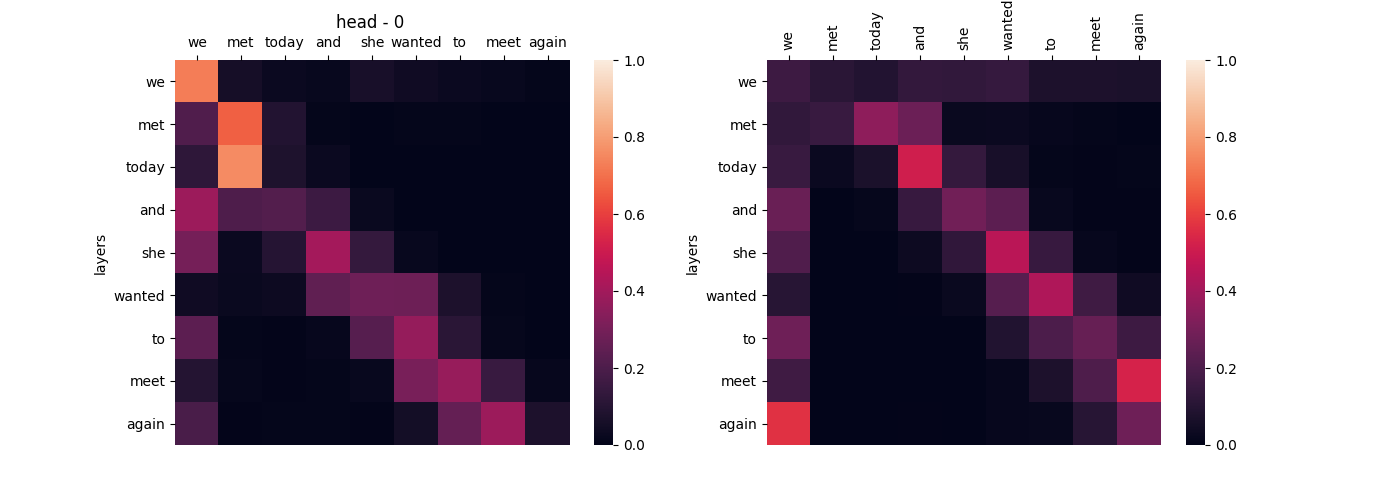
\includegraphics[width=1 
% 			\columnwidth]{attn.png}}
% 		\caption{Self Attention Framework}
% 		\label{fig:attn}
% 	\end{center}
% \end{figure*}

\begin{figure}[t]
	\centering
	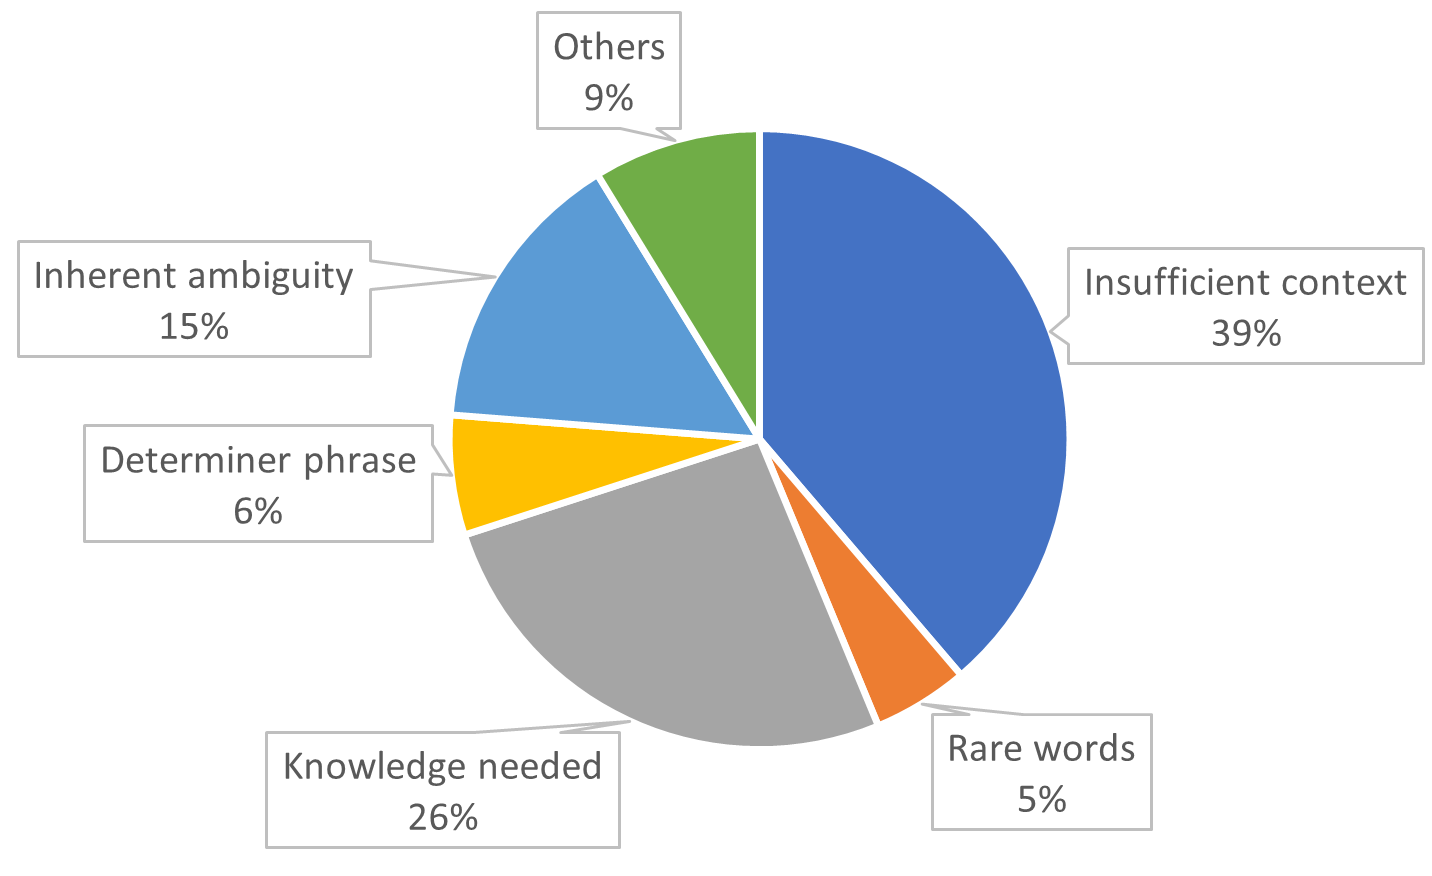
\includegraphics[width=0.9\columnwidth]{case_dist.png}
	\caption{Distribution of remaining errors on the test set.}
	\label{error_dist}
\end{figure}


\begin{figure*}[t]
	\centering
	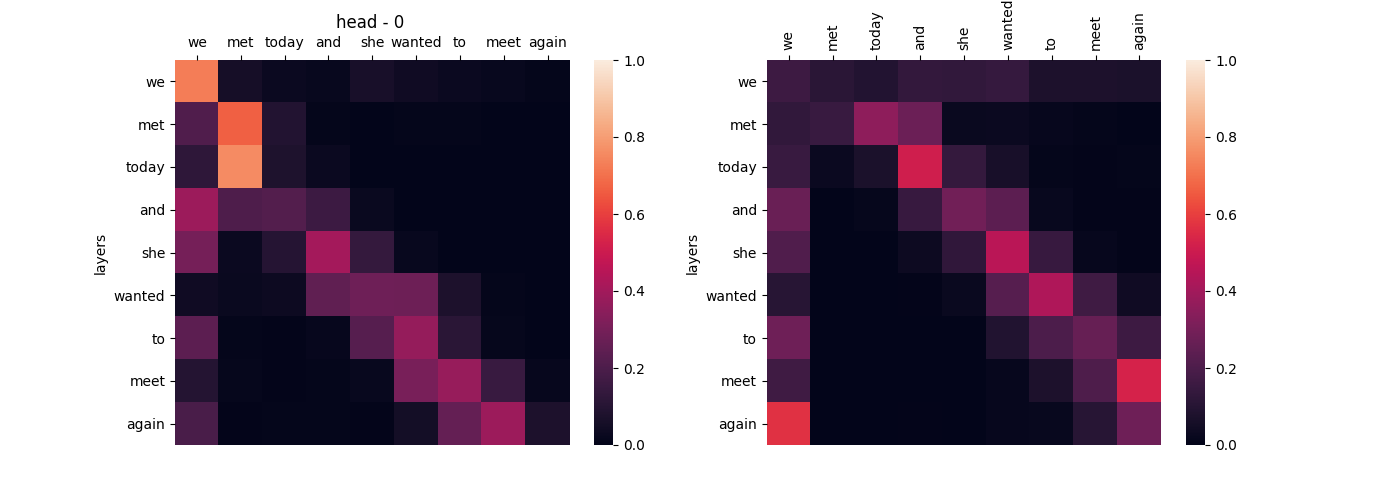
\includegraphics[width=2\columnwidth]{attn.png}
	\caption{Attention visualization heatmap for chemical }
	\label{fig:attn}
\end{figure*}

